% !TEX root =  ../../../thesis.tex
\section{Experimental Results}
\label{sec:automatic_training:experimentalResults}

\subsection{Convergence of AAM Automatic Construction}
\label{subsec:training}
Firstly, in order to create a facial shape PDM, we use 50 annotated images of
the LFPW database, appropriately selected to demonstrate various deformations
and expressions, and apply PCA. Note that one could also project shape
instances of a statistical 3D shape model~\cite{paysan20093d,booth20163d} to
the 2D plane. Then, we automatically build a facial AAM with the proposed method
(Fig.~\ref{fig:systemOverview}) using the images of LFPW and HELEN training
sets (2810 images in total). In order to perform the iteration between
generative and discriminative model, we split these images in two equal
disjoint subsets, each consisting of half of the images of each database, thus
405 and 1000 from LFPW and HELEN, respectively. We retrieve the bounding boxes
by using Google Picasa's face detection.

We execute the overall proposed methodology for 2 iterations in total, which
involves an iterative generative model automatic construction followed by a
discriminative model and then the final automatic generative model. Our
experiments show that the method converges quickly and only a single
application of the discriminative model is sufficient to move the generative
model to a satisfactory minimum. Figure~\ref{fig:generativeTraining_1}
plots the cost function vs. the number of iterations of the first generative
model training on the generative database, the initialization with the first
discriminative model (marked with an x) and the application of the final
generative model. As can be seen the application of the discriminative step
acts as a perturbation over the local optimum which in the end results to a
better solution (similar to random perturbations in Simulated Annealing).

\begin{figure}[!h]
  \centering
  \subfloat[Plot of the cost function per iteration. The marked point $\times$ denotes the beginning of the second iteration of the generative model.]{\includegraphics[width=0.72\linewidth]{figures/automatic_training/Training/overall/meanMSE.png}\label{fig:generativeTraining_1}}\\
  \subfloat[Plot of the respective point-to-point normalized RMSE.]{\includegraphics[width=0.72\linewidth]{figures/automatic_training/Training/overall/meanRMSE.png}\label{fig:generativeTraining_2}}
  \caption{Convergence of the automatic construction of AAM with a single application of the discriminative model. The convergence is shown with respect to the cost function minimization and the fitting accuracy.}
  \label{fig:generativeTraining}
\end{figure}
%

%
\begin{figure}[!h]
  \centering
  \includegraphics[width=0.72\linewidth]{figures/automatic_training/Training/overall/overallTraining.png}
  \caption{Automatic construction of AAM with a single application of the discriminative model. The plot shows the accuracy evolution of the generative database's shapes compared with their manual annotations.}
  \label{fig:overallTraining}
\end{figure}
%
%
\begin{figure}[!h]
  \centering
  \includegraphics[width=0.61\linewidth]{figures/automatic_training/Training/generative/subspaces.png}
  \caption{Automatic construction of AAM with a single application of the discriminative model.Visualization of the mean appearance and the three most important eigenvectors for the iterative automatically constructed AAM \emph{(top)} and the AAM trained on manual annotations \emph{(bottom)}.}
  \label{fig:generativeTrainingEigenvectors}
\end{figure}
%
Figure~\ref{fig:generativeTraining_2} plots the normalized RMSE over the number
of iterations for the generative database. The RMSE is the one defined in
Eq.~\ref{equ:error} with the face size as normalization constant
(Eq.~\ref{equ:error_normalization}). As can be seen, it monotonically
decreases. Furthermore, in Fig.~\ref{fig:overallTraining} we demonstrate the
evolution of the fitting curves of the generative database's shapes during this
training procedure compared with the manually annotated shapes.

Figure~\ref{fig:generativeTrainingEigenvectors} demonstrates the respective
evolution of the mean appearance and the three most important eigenvectors. The
last row demonstrates the subspace obtained from the PCA on the manual
annotations of the generative database. The figure shows that the resulting
facial appearance subspace gradually improves and isolates the outliers as
expected, due to the employment of the robust component analysis. This is
highlighted by the fact that the facial parts (eyes, nose, mouth etc.) can be
distinguished more clearly in the final eigentextures, as opposed to the
initial ones. The resulting appearance subspace is very similar to the
annotations-based one, even though we performed only two iterations.

Furthermore, Fig.~\ref{fig:shapesEvolution} shows the evolution of the fitted
shapes for eight images during the automatic building procedure. Starting from
the bounding boxes (first row), the final result of the last generative model
(last row) is very accurate. This figure also highlights the importance of the
discriminative model. Even though the fitted shapes that it provides are not
accurate, because its discriminative nature requires carefully annotated data,
however, it manages to move the generative model’s shapes from the point where
they stuck. We believe that the final fitted shapes shown at the last row of
Fig.~\ref{fig:shapesEvolution} are very impressive, given the automatic nature
of the proposed method. Moreover, Fig.~\ref{fig:worstShapes} shows the eight
fitted shapes with the worst RMSE error, that were estimated automatically with
the proposed procedure. As can be seen, even in the worst cases, the method
provides decent shapes.
%
\begin{figure}[!h]
  \centering
  \includegraphics[width=\linewidth]{figures/automatic_training/evolution/worst_8images_line5.png}
  \caption{The 8 worst fitted shapes during the automatic construction of AAM with a single application of the discriminative model.}
  \label{fig:worstShapes}
\end{figure}
%

%
\begin{figure}[!t]
  \centering
  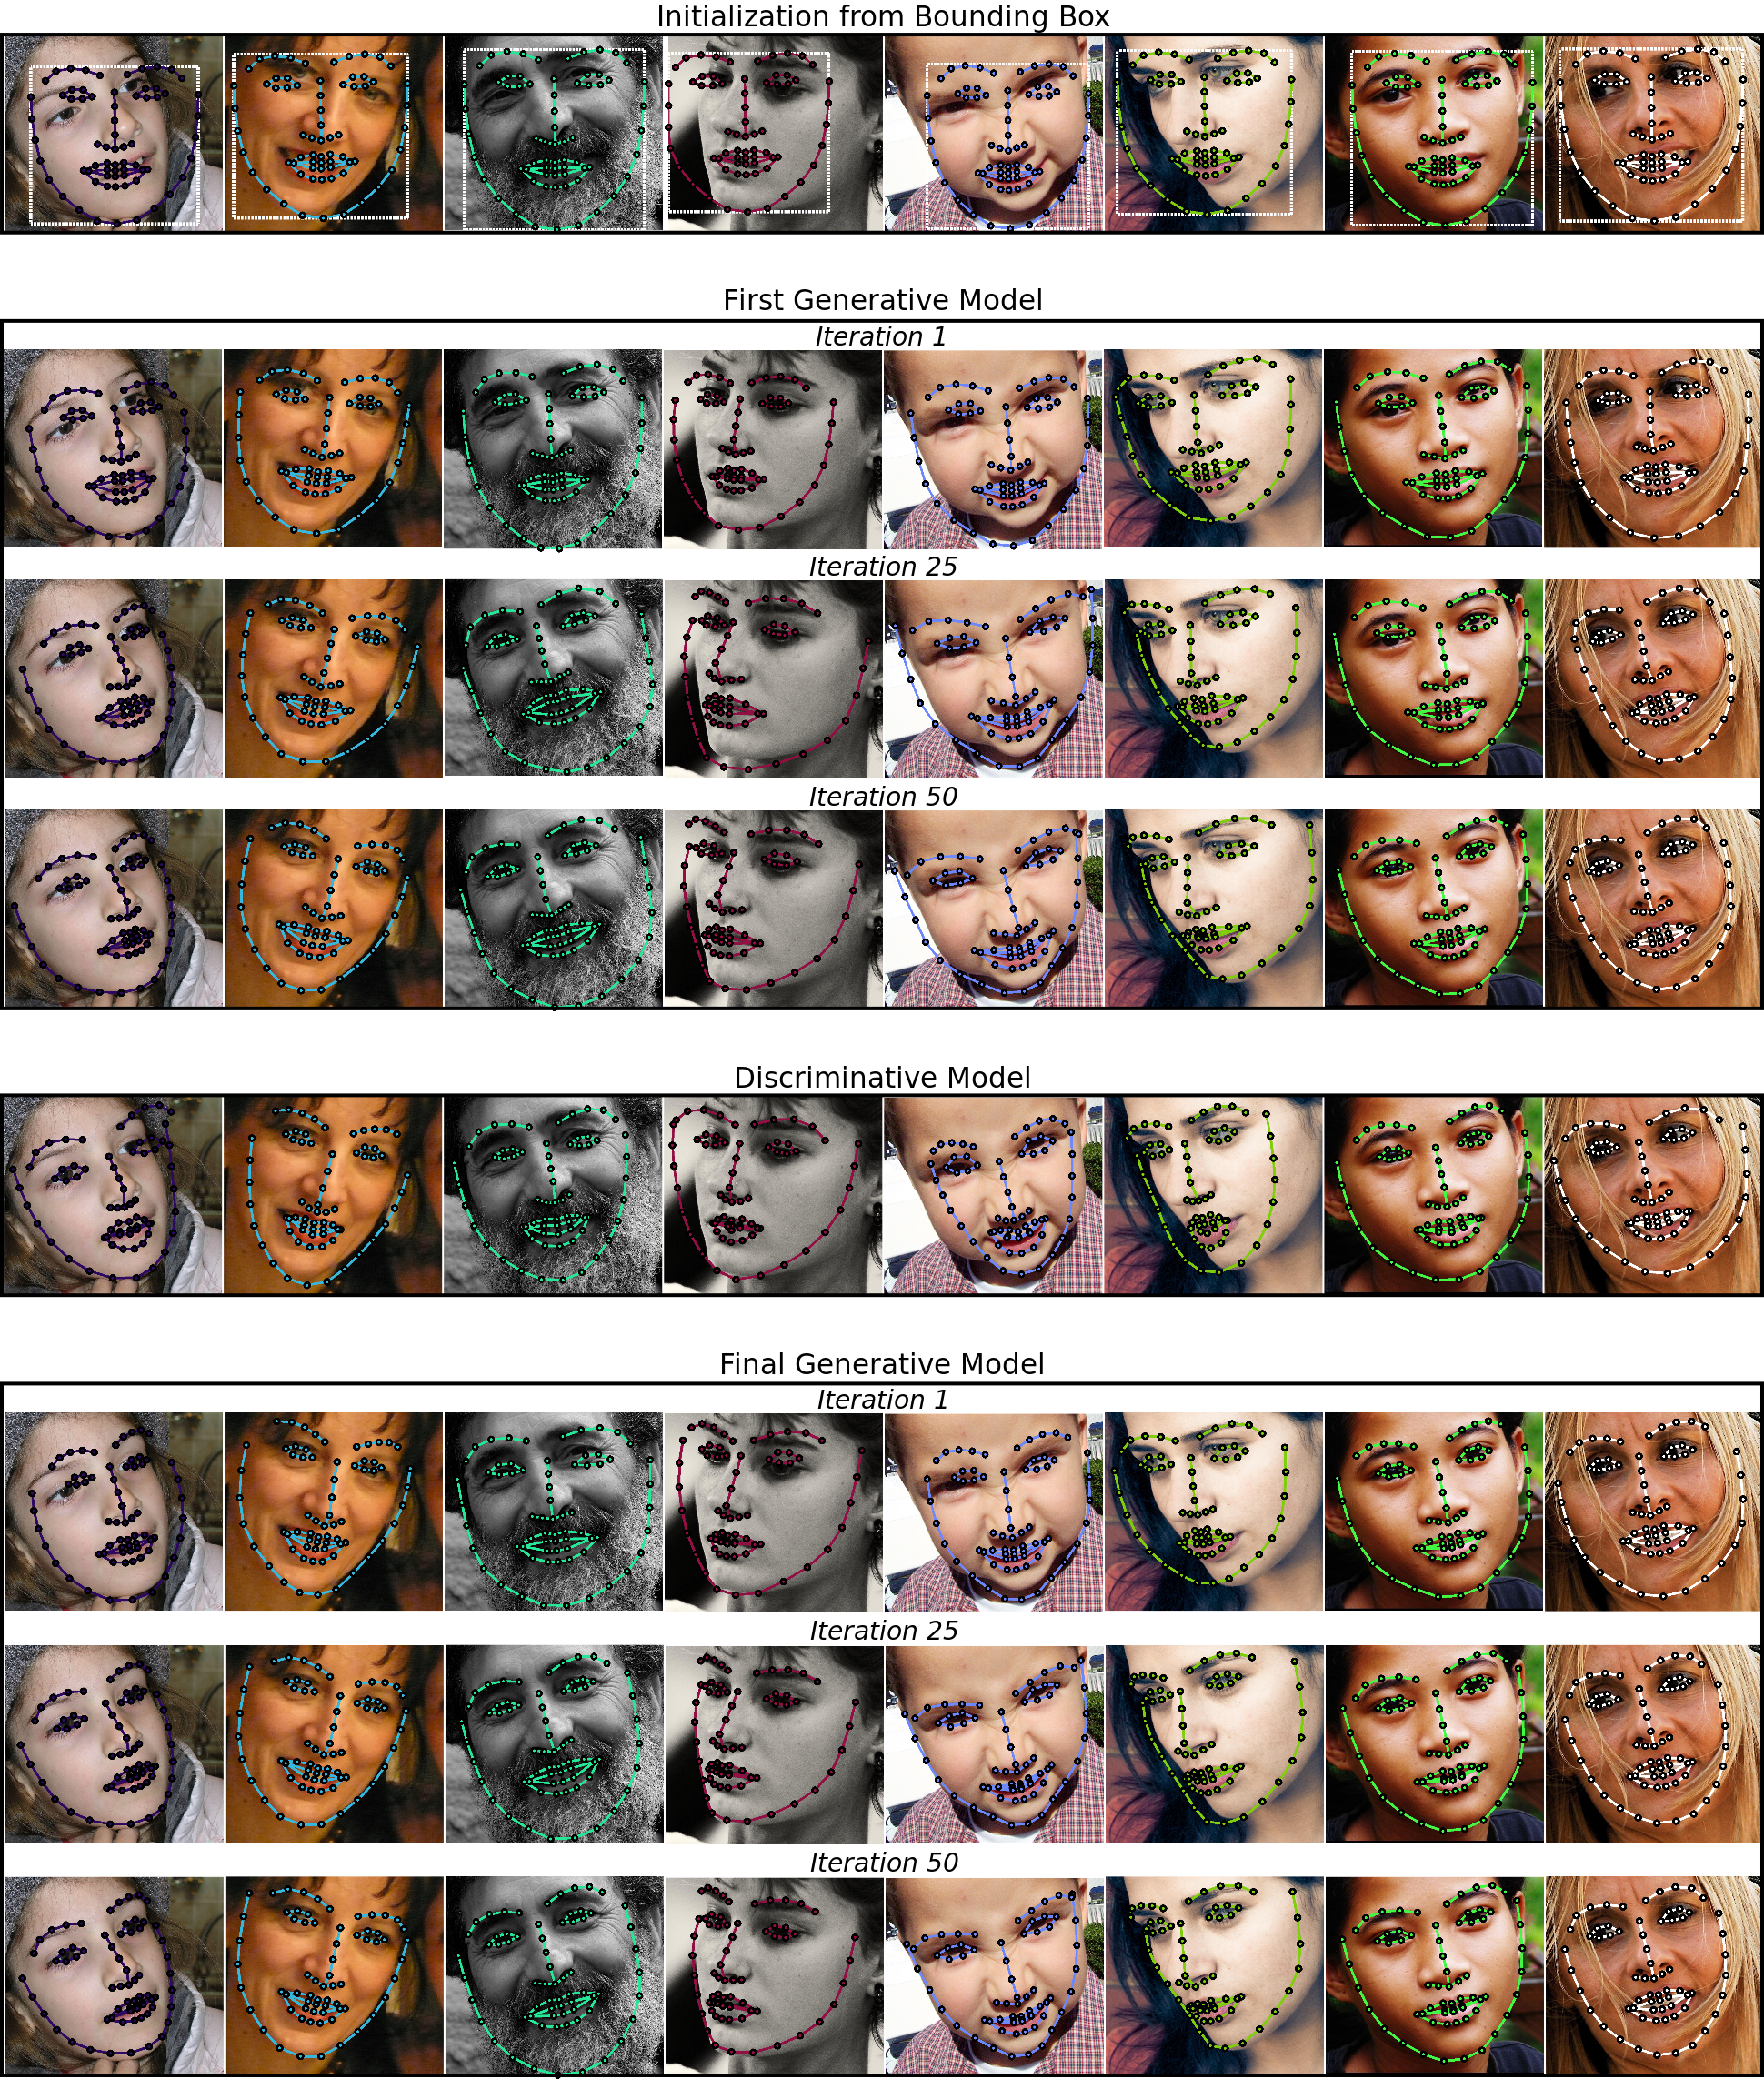
\includegraphics[width=\linewidth]{figures/automatic_training/evolution/8images_line5_2.png}
  \caption{Automatic construction of AAM with a single application of the discriminative model. The figures show the evolution of the fitted shapes for 8 images, starting from the bounding boxes. Each automatically trained generative model is performed for 50 iterations.}
  \label{fig:shapesEvolution}
\end{figure}
%

%
\begin{figure}[!t]
  \centering
  \includegraphics[width=0.58\linewidth]{figures/automatic_training/RESULTS/legend_dia.png}\\
  \subfloat[AFW database]{\includegraphics[width=0.72\linewidth]{figures/automatic_training/RESULTS/afw.png}\label{fig:results_1}}\\
  \subfloat[LFPW and HELEN testing databases]{\includegraphics[width=0.72\linewidth]{figures/automatic_training/RESULTS/helen.png}\label{fig:results_2}}
  \caption{Comparison of automatically constructed deformable models (generative and discriminative) with other models trained on manual annotations.}
\label{fig:results}
\end{figure}
%
\subsection{Comparison with Models Trained on Manual Annotations}
\label{subsec:comparison}
After completing the iterations demonstrated in
Figs.~\ref{fig:generativeTraining} and~\ref{fig:generativeTrainingEigenvectors},
we train a final generative and discriminative model on the 2810 images of the
union of both datasets. We compare the performance of our model with the
state-of-the-art method of Robust Discriminative Response Map Fitting (DRMF)
for Constrained Local Models~\cite{asthana2013robust} and the Deformable
Part-Based Models~\cite{zhu2012face}. For both methods, we use the
implementation provided by their authors, along with the pre-built models which
are discriminatively trained on the manual annotations of much larger datasets
than LFPW and HELEN datasets. Moreover, we compare with the generative and
discriminative AAMs trained on the manual annotations of LFPW and HELEN
trainsets. Figure~\ref{fig:results} shows the normalized RMSE curves on AFW and
the union of LFPW and HELEN testsets. Note that in both cases, we use Google
Picasa's face detection to extract the bounding boxes that initialize the
translation and scaling of the mean shape. The results show that our
automatically trained models have a very good performance and greatly
outperform the discriminative ones trained on manual annotations.

Finally, Figs.~\ref{fig:afw} and~\ref{fig:lfpwAndHelen} show some indicative
fitting results for the AFW dataset and the union of LFPW and HELEN databases,
respectively. Again, we strongly believe that these results are very promising,
especially considering the fact that our method’s models were constructed by
starting with just a bounding box per face.

%
\begin{figure}[!h]
  \centering
  \subfloat[Automatically trained generative model.]{
  \includegraphics[width=0.105\linewidth]{figures/automatic_training/RESULTS/AFWimages/Subject1_AutomaticGeberative.png}
  \includegraphics[width=0.105\linewidth]{figures/automatic_training/RESULTS/AFWimages/Subject3_AutomaticGeberative.png}
  \includegraphics[width=0.105\linewidth]{figures/automatic_training/RESULTS/AFWimages/Subject4_AutomaticGeberative.png}
  \includegraphics[width=0.105\linewidth]{figures/automatic_training/RESULTS/AFWimages/Subject7_AutomaticGeberative.png}
  \includegraphics[width=0.105\linewidth]{figures/automatic_training/RESULTS/AFWimages/Subject10_AutomaticGeberative.png}
  \includegraphics[width=0.105\linewidth]{figures/automatic_training/RESULTS/AFWimages/Subject11_AutomaticGeberative.png}
  \includegraphics[width=0.105\linewidth]{figures/automatic_training/RESULTS/AFWimages/Subject12_AutomaticGeberative.png}
  \includegraphics[width=0.105\linewidth]{figures/automatic_training/RESULTS/AFWimages/Subject13_AutomaticGeberative.png}
  \includegraphics[width=0.105\linewidth]{figures/automatic_training/RESULTS/AFWimages/Subject14_AutomaticGeberative.png}
  %\includegraphics[width=0.105\linewidth]{figures/automatic_training/RESULTS/AFWimages/Subject15_AutomaticGeberative.png}
  }

  \subfloat[Generative model trained on manual annotations.]{
  \includegraphics[width=0.105\linewidth]{figures/automatic_training/RESULTS/AFWimages/Subject1_AnnotationsGenerative.png}
  \includegraphics[width=0.105\linewidth]{figures/automatic_training/RESULTS/AFWimages/Subject3_AnnotationsGenerative.png}
  \includegraphics[width=0.105\linewidth]{figures/automatic_training/RESULTS/AFWimages/Subject4_AnnotationsGenerative.png}
  \includegraphics[width=0.105\linewidth]{figures/automatic_training/RESULTS/AFWimages/Subject7_AnnotationsGenerative.png}
  \includegraphics[width=0.105\linewidth]{figures/automatic_training/RESULTS/AFWimages/Subject10_AnnotationsGenerative.png}
  \includegraphics[width=0.105\linewidth]{figures/automatic_training/RESULTS/AFWimages/Subject11_AnnotationsGenerative.png}
  \includegraphics[width=0.105\linewidth]{figures/automatic_training/RESULTS/AFWimages/Subject12_AnnotationsGenerative.png}
  \includegraphics[width=0.105\linewidth]{figures/automatic_training/RESULTS/AFWimages/Subject13_AnnotationsGenerative.png}
  \includegraphics[width=0.105\linewidth]{figures/automatic_training/RESULTS/AFWimages/Subject14_AnnotationsGenerative.png}
  %\includegraphics[width=0.105\linewidth]{figures/automatic_training/RESULTS/AFWimages/Subject15_AnnotationsGenerative.png}
  }

  \subfloat[Automatically trained discriminative model.]{
  \includegraphics[width=0.105\linewidth]{figures/automatic_training/RESULTS/AFWimages/Subject1_AutomaticDiscriminative.png}
  \includegraphics[width=0.105\linewidth]{figures/automatic_training/RESULTS/AFWimages/Subject3_AutomaticDiscriminative.png}
  \includegraphics[width=0.105\linewidth]{figures/automatic_training/RESULTS/AFWimages/Subject4_AutomaticDiscriminative.png}
  \includegraphics[width=0.105\linewidth]{figures/automatic_training/RESULTS/AFWimages/Subject7_AutomaticDiscriminative.png}
  \includegraphics[width=0.105\linewidth]{figures/automatic_training/RESULTS/AFWimages/Subject10_AutomaticDiscriminative.png}
  \includegraphics[width=0.105\linewidth]{figures/automatic_training/RESULTS/AFWimages/Subject11_AutomaticDiscriminative.png}
  \includegraphics[width=0.105\linewidth]{figures/automatic_training/RESULTS/AFWimages/Subject12_AutomaticDiscriminative.png}
  \includegraphics[width=0.105\linewidth]{figures/automatic_training/RESULTS/AFWimages/Subject13_AutomaticDiscriminative.png}
  \includegraphics[width=0.105\linewidth]{figures/automatic_training/RESULTS/AFWimages/Subject14_AutomaticDiscriminative.png}
  %\includegraphics[width=0.105\linewidth]{figures/automatic_training/RESULTS/AFWimages/Subject15_AutomaticDiscriminative.png}
  }

  \subfloat[Discriminative model trained on manual annotations.]{
  \includegraphics[width=0.105\linewidth]{figures/automatic_training/RESULTS/AFWimages/Subject1_AnnotationsDiscriminative.png}
  \includegraphics[width=0.105\linewidth]{figures/automatic_training/RESULTS/AFWimages/Subject3_AnnotationsDiscriminative.png}
  \includegraphics[width=0.105\linewidth]{figures/automatic_training/RESULTS/AFWimages/Subject4_AnnotationsDiscriminative.png}
  \includegraphics[width=0.105\linewidth]{figures/automatic_training/RESULTS/AFWimages/Subject7_AnnotationsDiscriminative.png}
  \includegraphics[width=0.105\linewidth]{figures/automatic_training/RESULTS/AFWimages/Subject10_AnnotationsDiscriminative.png}
  \includegraphics[width=0.105\linewidth]{figures/automatic_training/RESULTS/AFWimages/Subject11_AnnotationsDiscriminative.png}
  \includegraphics[width=0.105\linewidth]{figures/automatic_training/RESULTS/AFWimages/Subject12_AnnotationsDiscriminative.png}
  \includegraphics[width=0.105\linewidth]{figures/automatic_training/RESULTS/AFWimages/Subject13_AnnotationsDiscriminative.png}
  \includegraphics[width=0.105\linewidth]{figures/automatic_training/RESULTS/AFWimages/Subject14_AnnotationsDiscriminative.png}
  %\includegraphics[width=0.105\linewidth]{figures/automatic_training/RESULTS/AFWimages/Subject15_AnnotationsDiscriminative.png}
  }

  \caption{Fitting results on AFW database.}
  \label{fig:afw}
\end{figure}
%

%
\begin{figure}[!t]
  \centering
  \subfloat[Automatically trained generative model.]{
  \includegraphics[width=0.105\linewidth]{figures/automatic_training/RESULTS/LFPWandHelenImages/Subject3_AutomaticGeberative.png}
  \includegraphics[width=0.105\linewidth]{figures/automatic_training/RESULTS/LFPWandHelenImages/Subject5_AutomaticGeberative.png}
  \includegraphics[width=0.105\linewidth]{figures/automatic_training/RESULTS/LFPWandHelenImages/Subject110_AutomaticGeberative.png}
  \includegraphics[width=0.105\linewidth]{figures/automatic_training/RESULTS/LFPWandHelenImages/Subject7_AutomaticGeberative.png}
  \includegraphics[width=0.105\linewidth]{figures/automatic_training/RESULTS/LFPWandHelenImages/Subject8_AutomaticGeberative.png}
  \includegraphics[width=0.105\linewidth]{figures/automatic_training/RESULTS/LFPWandHelenImages/Subject9_AutomaticGeberative.png}
  \includegraphics[width=0.105\linewidth]{figures/automatic_training/RESULTS/LFPWandHelenImages/Subject10_AutomaticGeberative.png}
  \includegraphics[width=0.105\linewidth]{figures/automatic_training/RESULTS/LFPWandHelenImages/Subject33_AutomaticGeberative.png}
  \includegraphics[width=0.105\linewidth]{figures/automatic_training/RESULTS/LFPWandHelenImages/Subject55_AutomaticGeberative.png}
  }

  \subfloat[Generative model trained on manual annotations.]{
  \includegraphics[width=0.105\linewidth]{figures/automatic_training/RESULTS/LFPWandHelenImages/Subject3_AnnotationsGenerative.png}
  \includegraphics[width=0.105\linewidth]{figures/automatic_training/RESULTS/LFPWandHelenImages/Subject5_AnnotationsGenerative.png}
  \includegraphics[width=0.105\linewidth]{figures/automatic_training/RESULTS/LFPWandHelenImages/Subject110_AnnotationsGenerative.png}
  \includegraphics[width=0.105\linewidth]{figures/automatic_training/RESULTS/LFPWandHelenImages/Subject7_AnnotationsGenerative.png}
  \includegraphics[width=0.105\linewidth]{figures/automatic_training/RESULTS/LFPWandHelenImages/Subject8_AnnotationsGenerative.png}
  \includegraphics[width=0.105\linewidth]{figures/automatic_training/RESULTS/LFPWandHelenImages/Subject9_AnnotationsGenerative.png}
  \includegraphics[width=0.105\linewidth]{figures/automatic_training/RESULTS/LFPWandHelenImages/Subject10_AnnotationsGenerative.png}
  \includegraphics[width=0.105\linewidth]{figures/automatic_training/RESULTS/LFPWandHelenImages/Subject33_AnnotationsGenerative.png}
  \includegraphics[width=0.105\linewidth]{figures/automatic_training/RESULTS/LFPWandHelenImages/Subject55_AnnotationsGenerative.png}
  }

  \subfloat[Automatically trained discriminative model.]{
  \includegraphics[width=0.105\linewidth]{figures/automatic_training/RESULTS/LFPWandHelenImages/Subject3_AutomaticDiscriminative.png}
  \includegraphics[width=0.105\linewidth]{figures/automatic_training/RESULTS/LFPWandHelenImages/Subject5_AutomaticDiscriminative.png}
  \includegraphics[width=0.105\linewidth]{figures/automatic_training/RESULTS/LFPWandHelenImages/Subject110_AutomaticDiscriminative.png}
  \includegraphics[width=0.105\linewidth]{figures/automatic_training/RESULTS/LFPWandHelenImages/Subject7_AutomaticDiscriminative.png}
  \includegraphics[width=0.105\linewidth]{figures/automatic_training/RESULTS/LFPWandHelenImages/Subject8_AutomaticDiscriminative.png}
  \includegraphics[width=0.105\linewidth]{figures/automatic_training/RESULTS/LFPWandHelenImages/Subject9_AutomaticDiscriminative.png}
  \includegraphics[width=0.105\linewidth]{figures/automatic_training/RESULTS/LFPWandHelenImages/Subject10_AutomaticDiscriminative.png}
  \includegraphics[width=0.105\linewidth]{figures/automatic_training/RESULTS/LFPWandHelenImages/Subject33_AutomaticDiscriminative.png}
  \includegraphics[width=0.105\linewidth]{figures/automatic_training/RESULTS/LFPWandHelenImages/Subject55_AutomaticDiscriminative.png}
  }

  \subfloat[Discriminative model trained on manual annotations.]{
  \includegraphics[width=0.105\linewidth]{figures/automatic_training/RESULTS/LFPWandHelenImages/Subject3_AnnotationsDiscriminative.png}
  \includegraphics[width=0.105\linewidth]{figures/automatic_training/RESULTS/LFPWandHelenImages/Subject5_AnnotationsDiscriminative.png}
  \includegraphics[width=0.105\linewidth]{figures/automatic_training/RESULTS/LFPWandHelenImages/Subject110_AnnotationsDiscriminative.png}
  \includegraphics[width=0.105\linewidth]{figures/automatic_training/RESULTS/LFPWandHelenImages/Subject7_AnnotationsDiscriminative.png}
  \includegraphics[width=0.105\linewidth]{figures/automatic_training/RESULTS/LFPWandHelenImages/Subject8_AnnotationsDiscriminative.png}
  \includegraphics[width=0.105\linewidth]{figures/automatic_training/RESULTS/LFPWandHelenImages/Subject9_AnnotationsDiscriminative.png}
  \includegraphics[width=0.105\linewidth]{figures/automatic_training/RESULTS/LFPWandHelenImages/Subject10_AnnotationsDiscriminative.png}
  \includegraphics[width=0.105\linewidth]{figures/automatic_training/RESULTS/LFPWandHelenImages/Subject33_AnnotationsDiscriminative.png}
  \includegraphics[width=0.105\linewidth]{figures/automatic_training/RESULTS/LFPWandHelenImages/Subject55_AnnotationsDiscriminative.png}
  }

  \caption{Fitting results on LFPW and HELEN testing databases.}
  \label{fig:lfpwAndHelen}
\end{figure}
